% 結果の章（数値は 図/values.tex と 図/tab_*.tex から。手で書かない）

% ============================================================
\chapter{再現の判定}\label{ch:replication}

\begin{table}[H]
\centering\small
\caption{S1〜S4 の主な検定：元の標本と新しい標本}
\label{tab:replication}
\begin{adjustbox}{max width=\linewidth}
\begin{tabular}{@{}llrrl@{}}
\toprule
実験 & 主な数字 & 元の標本 & 新しい標本 & 判定 \\
\midrule
S1：ドリフトの予測（ChronoGPT＋リッジ → 2〜60 日の超過リターン） & 係数（bp/SD） & \V{oSonec} & \V{rSonec} & \textbf{\V{RSone}} \\
 & $t$ & \V{oSonet} & \V{rSonet} & \\
 & 並べ替えの片側 $p$ & \V{oSoneperm} & \V{rSoneperm} & \\
S2：変動率の予測（ChronoGPT＋リッジ → 2〜60 日の変動率） & 係数（\%/SD） & \V{oStwoc} & \V{rStwoc} & \textbf{\V{RStwo}} \\
 & $t$ & \V{oStwot} & \V{rStwot} & \\
 & 並べ替えの片側 $p$ & \V{oStwoperm} & \V{rStwoperm} & \\
S3：文章のリスクの点数で共分散を補正（B → C） & 偏り $b$（B） & \V{oSthreeb} & \V{rSthreeb} & \textbf{\V{RSthree}}（効果なし） \\
 & 偏り $b$（C） & \V{oSthreec} & \V{rSthreec} & \\
 & 片側 $p$ & \V{oSthreep} & \V{rSthreep} & \\
S4：TE の上限の校正（B → B＋校正） & $g$（B） & \V{oSfourb} & \V{rSfourb} & \textbf{\V{RSfour}} \\
 & $g$（B＋校正） & \V{oSfourc} & \V{rSfourc} & \\
 & 実現の TE（B＋校正） & \V{oSfourte} & \V{rSfourte} & \\
 & 片側 $p$ & \V{oSfourp} & \V{rSfourp} & \\
\bottomrule
\end{tabular}
\end{adjustbox}
\end{table}

評価した発表は、新しい標本で \V{neval} 件（元の標本は \V{nevalorig} 件）、gpt-4o-mini の期間（2024 年以降）は \V{nevalgpt} 件。偏り $b$ = 日々の（BLM − 相手）÷ 事前の TE の 2 乗平均の平方根、$g$ = 日々の（BLM − 相手）÷（3\%$/\sqrt{252}$）の 2 乗平均の平方根（どちらも 1 なら見積もりどおり）。

\begin{keybox}[結果]
\textbf{4 つのうち \V{nreplicated} つが再現した}。
\begin{itemize}
\item \textbf{S1（ドリフト）}：係数は元の \V{oSonec}bp から \V{rSonec}bp に小さくなったが、$t$ = \V{rSonet}、並べ替えの $p$ = \V{rSoneperm} で、同じ基準を満たした。
\item \textbf{S2（変動率）}：\V{rStwoc}\%/SD（$t$ = \V{rStwot}）。元より小さいが、同じ向きではっきりしている。
\item \textbf{S3（文章による共分散の補正）}：元と同じく、補正しても偏りは変わらなかった（効果がないことが再現した）。
\item \textbf{S4（TE の校正）}：再現しなかった。新しい標本では偏りが \V{rSfourb} と大きく（元は \V{oSfourb}）、校正しても \V{rSfourc}（実現の TE \V{rSfourte}）にしか下がらなかった。原因は \chapref{ch:explore} の探索で調べた。
\end{itemize}
\end{keybox}

\begin{figure}[H]
\centering
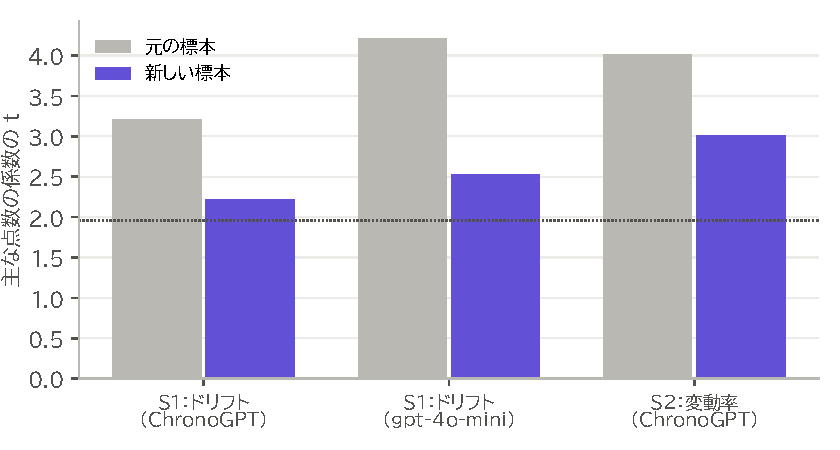
\includegraphics[width=0.72\linewidth]{coef.pdf}
\caption{主な点数の係数の $t$。点線は 1.96。S1 の gpt-4o-mini は副次の検定（2024 年以降）。}
\label{fig:coef}
\end{figure}

gpt-4o-mini の読み取り（学習なし）も、新しい標本でドリフトを予測した（\V{rgptc}bp/SD、$t$ = \V{rgptt}。元は \V{ogptc}bp、$t$ = \V{ogptt}）。

S1 の副次の月次のポートフォリオ（点数の上位 5 分の 1 を浮動株時価総額で持つ、片道 0.3\% の費用の後）は、元の標本で月 \V{oport}（$t$ = \V{oportt}）、新しい標本で月 \V{rport}（$t$ = \V{rportt}）で、どちらも比べる相手との差ははっきりしなかった。

% ============================================================
\chapter{新しい主な検定（R-BLM）}\label{ch:rblm}

\begin{keybox}[結果]
事前登録の基準では\textbf{\V{Bverdict}された}。2015 年末から四半期ごとの BLM（ChronoGPT＋リッジ、共分散 B、TE の校正あり）の、2017 年以降 \V{Bdays} 日の比べる相手との差は年 \V{Bex}（95\% 区間 [\V{Blo}, \V{Bhi}]、片側 $p$ \V{Bp}）、情報レシオ \V{Bir}。

\textbf{ただし実現の TE は \V{Bte} で、約束の 3\% の約 3 倍だった}。この差の多くは 1 日のデータの誤りから来ている（\chapref{ch:explore}）。
\end{keybox}

\begin{table}[H]
\centering\small
\caption{BLM と比べる相手の差（年率、評価する日）。主な検定は 1 行目。ほかは副次（判定には使わない）。元の標本の列は、R1 の事前登録を書いた時点で一度計算していた探索の値}
\label{tab:blm}
\tabin{blm}
\end{table}

\begin{figure}[H]
\centering
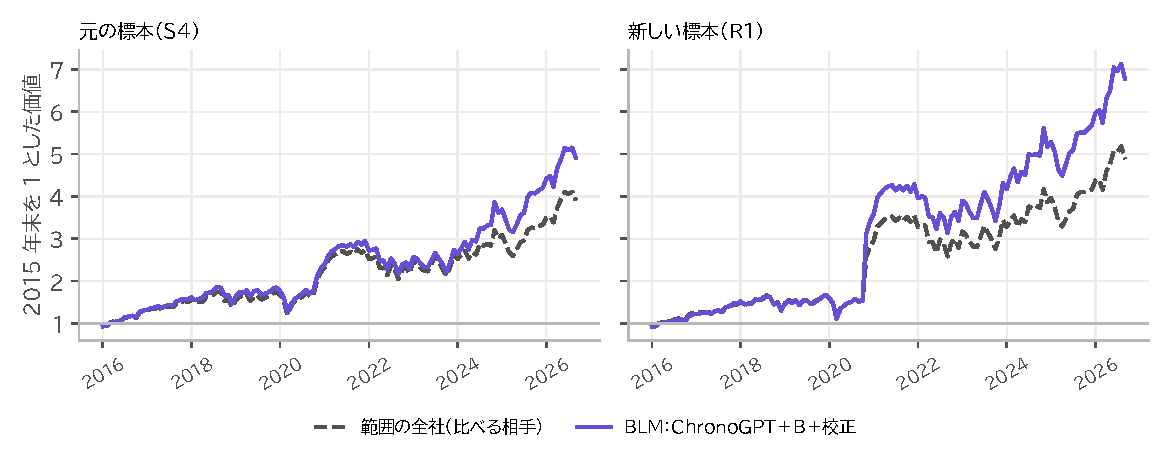
\includegraphics[width=\linewidth]{paths.pdf}
\caption{2015 年末を 1 とした推移（四半期ごと、ChronoGPT＋リッジ、共分散 B、TE の校正あり）。新しい標本の 2020 年 11 月の跳ね上がりの多くは、比べる相手にも BLM にも入っている株価の誤り（\chapref{ch:explore}）。}
\label{fig:paths}
\end{figure}

最終の値は、元の標本で BLM \V{ofinal}・相手 \V{oband}、新しい標本で BLM \V{rfinal}・相手 \V{rband}。

% ============================================================
\chapter{探索：TE が約束の約 3 倍になった理由}\label{ch:explore}

\textbf{この章は事前登録していない}。R1 の結果を見た後に、新しい標本で実現の TE が大きかった理由を調べた（\code{experiments/R1\_replication/explore.py}、結果は \code{results/explore\_orig.json}・\code{explore\_rep.json}）。ここの数字で、前の章の判定は変えない。

\section{1 日の寄与}

\begin{figure}[H]
\centering
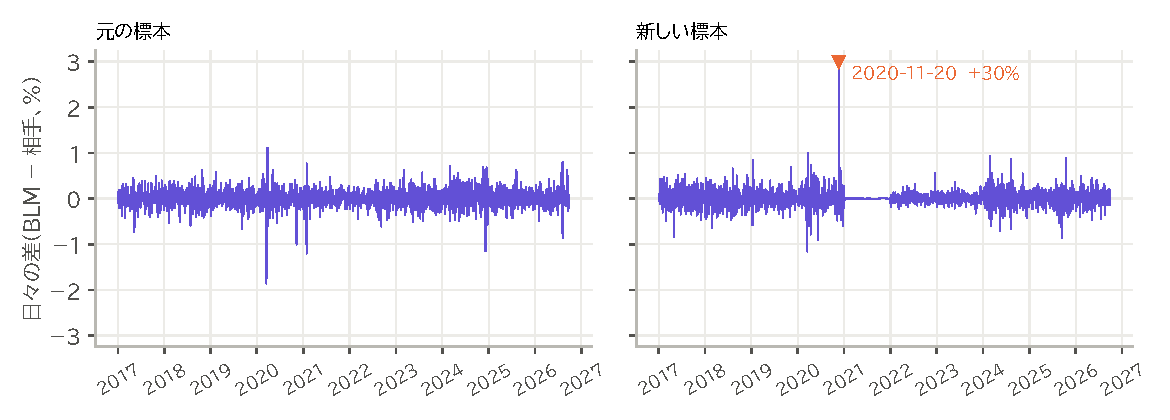
\includegraphics[width=\linewidth]{active.pdf}
\caption{日々の差（BLM − 比べる相手、\%）。2017 年以降、四半期ごと、共分散 B、TE の校正あり。$\pm$3\% を超える日は端に印を付けた。}
\label{fig:active}
\end{figure}

新しい標本では、\V{rtopday} の 1 日に、BLM と相手の差が \V{rtopactive} 開いた。日々の差の 2 乗の合計のうち、いちばん大きい 5 日が占める割合は、新しい標本で \V{rshareBcal}（元の標本は \V{oshareBcal}）。この 5 日を除くと、偏り $g$ は次のようになる。

\begin{table}[H]
\centering\small
\caption{偏り $g$（2017 年以降、四半期ごと）と、いちばん大きい 5 日を除いた値}
\label{tab:top5}
\begin{tabular}{@{}lrrrr@{}}
\toprule
 & \multicolumn{2}{c}{元の標本} & \multicolumn{2}{c}{新しい標本} \\
\cmidrule(lr){2-3}\cmidrule(lr){4-5}
共分散 & $g$ & 5 日を除く & $g$ & 5 日を除く \\
\midrule
A（補正なし） & \V{ogA} & \V{ogwoA} & \V{rgA} & \V{rgwoA} \\
B（株価で補正） & \V{ogB} & \V{ogwoB} & \V{rgB} & \V{rgwoB} \\
B＋校正 & \V{ogBcal} & \V{ogwoBcal} & \V{rgBcal} & \V{rgwoBcal} \\
\bottomrule
\end{tabular}
\end{table}

5 日を除くと、新しい標本の偏りは元の標本と同じくらいになり、校正すると 1 を下回った。

\section{原因：破産から再出発した会社の株価のつなぎ}

その日に大きく動いたのは CHRD（今の Chord Energy。2020 年当時は Oasis Petroleum）だった。Oasis は 2020 年に連邦破産法 11 条の手続きに入り、2020 年 11 月に新しい株で再出発した。古い株は取り消されて新しい株が発行されたので、古い株を持っていた人の資産が 1 日で 250 倍になったわけではない。ところが yfinance は、古い株の最後の価格（0.12 ドル）に新しい株の最初の価格（31 ドル）をそのままつないでいて、調整後終値の日々のリターンは \V{rtopday} に約 +25{,}700\% になっていた。

BLM はこの銘柄を相手より約 0.1\% 多く持っていたので、この 1 日で差が大きく開いた。比べる相手も浮動株時価総額でこの銘柄を持っていたので、相手の価値も同じ日に跳ね上がった（\figref{fig:paths}）。さらに、TE の校正は過去 756 日の偏りで上限を割るので、この 1 日が過去 756 日に入っていた 2020 年 12 月から 2023 年 9 月まで（12 回のリバランス、約 3 年）、上限は下限の 1\% に張り付き、BLM の動きは小さくなった（\figref{fig:active}）。

同じような日は、両方の標本にあった。

\begin{table}[H]
\centering\small
\caption{標本の会社の日々のリターン（調整後終値、2015 年以降）のうち、ありえない大きさのもの}
\label{tab:extreme}
\begin{tabular}{@{}lrr@{}}
\toprule
 & 元の標本 & 新しい標本 \\
\midrule
会社 × 日の数 & \V{onstockdays} & \V{rnstockdays} \\
$+$300\% を超える日 & \V{onup} & \V{rnup} \\
$+$100\% を超える日 & \V{onupone} & \V{rnupone} \\
$-$80\% を下回る日 & \V{ondown} & \V{rndown} \\
\bottomrule
\end{tabular}
\end{table}

いちばん大きいもの：元の標本は \V{obigjumps}、新しい標本は \V{rbigjumps}。破産からの再出発のつなぎのほか、1 日で何十倍にもなって翌日に元へ戻る、価格の乱れもあった。

\section{ありえないリターンを除いた計算}

S4 の 2015 年末から四半期ごとのポートフォリオを、日々のリターンのうちしきい値を超えるものを欠け（S4 は欠けた価格を 0\% と数える）として、計算し直した。しきい値は、計算する前に 3 通り決めた（主：$+$300\% 超か $-$80\% 未満）。そのままの計算は S4 の値と\V{rreproduces}（元の標本でも\V{oreproduces}）。

\begin{table}[H]
\centering\small
\caption{ありえない日々のリターンを除いた計算（2017 年以降、四半期ごと、ChronoGPT＋リッジ）。最終の値は 2015 年末を 1 とした 2026 年 9 月末の値}
\label{tab:explore}
\tabin{explore}
\end{table}

\begin{keybox}[探索の結果]
\begin{itemize}
\item 主のしきい値で除くと（新しい標本で \V{rnremoved} 個の会社 × 日）、新しい標本の B＋校正の偏りは $g$ = \V{rmainBcalg}（実現の TE \V{rmainBcalte}）になり、約束の 3\% に近づいた。比べる相手との差は年 \V{rmainBcalex}（95\% 区間 [\V{rmainBcallo}, \V{rmainBcalhi}]、片側 $p$ \V{rmainBcalp}）、情報レシオ \V{rmainBcalir}。
\item 元の標本では、除いても結果はほとんど変わらなかった（差は年 \V{omainBcalex}、片側 $p$ \V{omainBcalp}、$g$ = \V{omainBcalg}）。
\item \textbf{誤りを除くと、新しい標本でも TE の校正は効いた}。偏り $g$ は、校正なしの B で \V{rmainBg}、B＋校正で \V{rmainBcalg}（元の標本は \V{omainBg} → \V{omainBcalg}）。S4 が再現しなかったのは、主にこの種の誤りのためだった。
\item 比べる相手の最終の値も、新しい標本ではそのままの \V{rnoneband} から \V{rmainband} に下がった。2020 年 11 月の跳ね上がりの多くが誤りだったことを裏づける。
\item つまり、R-BLM の年 \V{Bex} の多くは株価の誤りから来ていた。誤りを除いた後の値が、この BLM の成績の、より正直な見積もりである。ただし、これは結果を見た後の分析なので、別の標本か別の期間で、誤りを除く手順を先に決めて確かめ直す必要がある。
\item ほかの 2 つのしきい値でも、結論は同じ向きだった（\tabref{tab:explore}）。最適化が解けなかったリバランスは、比べる相手の比率のままにした（S4 が解けないときと同じ扱い）。
\end{itemize}
\end{keybox}

% ============================================================
\chapter{まとめ}\label{ch:summary}

\begin{itemize}
\item \textbf{決算発表文の読み取りが、小型株の発表後のドリフトと変動率を予測することは、別の 1,000 社でも再現した}（S1・S2）。係数は元の標本より小さかった。
\item \textbf{文章のリスクの点数で共分散を補正しても、TE の見積もりは良くならない}ことも再現した（S3）。
\item \textbf{TE の校正（S4）と R-BLM は、株価データの誤り 1 日に大きく左右された}。事前登録の判定（S4 は再現しない、R-BLM は支持）はそのまま記録するが、どちらも誤りの影響を受けた結果である。
\item \textbf{誤りを除くと（探索）}、TE の校正は両方の標本で効き（実現の TE 約 3\%）、BLM は両方の標本で比べる相手を年 約 3\% 上回った（新しい標本 \V{rmainBcalex}、元の標本 \V{omainBcalex}）。事前登録の値（年 \V{Bex}）の約半分は誤りによる上乗せだった。
\item \textbf{これからの手順}：小型株の株価は、計算の前に、ありえない日々のリターン（破産からの再出発のつなぎ、1 日だけの乱れ）を取り除く。その規則を事前登録に書いてから、BLM の検定をやり直す。
\end{itemize}
